\documentclass[hyperref={pdfpagemode=FullScreen, colorlinks=false}]{beamer}

\usepackage{tikz}
\usetikzlibrary{patterns}
\usetikzlibrary{decorations.pathmorphing}

\usepackage{selinput}			% Inputencoding
	\SelectInputMappings{adieresis={ä}, germandbls={ß}, Euro={€}}
\usepackage[T1]{fontenc}		% Fontencoding
%
\usepackage{pifont}
\usepackage{csquotes,siunitx}			% Anführungszeichen; wird von biblatex gewünscht
\usepackage[backend=biber,citestyle=alphabetic,uniquelist=false]{biblatex}	% Literatur formatieren
\addbibresource{bodendynamik.bib}	% Literaturdatenbank
\usepackage{caption} 
\usepackage{subfig}
\usepackage{comment}
%%%%%%%%%%%%%%%%%%%%%%%%%%%%%%%%%%%%%%%%%%%%%%%%%%%%%%%%%%%%%%%%%%%%%%%%%%%%%%%%%%%%%%%%%%%%%%%%%%%%%%%
% Thema für Präsentation
\usetheme[fusszeile=ernstcolor,sprache=ngerman,seite=letzte,
verhaeltnis=16:10,
hausschrift=false,
navigation=false,
titelseite=blau]{TUBAF}

\TUBAFZweitlogo{
\includegraphics{fig_pdf/UFZ_logo_inv.pdf}}

%%%%%%%%%%%%%%%%%%%%%%%%%%%%%%%%%%%%%%%%%%%%%%%%%%%%%%%%%%%%%%%%%%%%%%%%%%%%%%%%%%%%%%%%%%%%%%%%%%%%%%%
% Optionen für Anmerkungen
\mode<presentation>{%
\setbeameroption{hide notes}				% keine Notizen (default)
%\setbeameroption{show notes}				% Notizen und Frames gemischt
%\setbeameroption{show only notes}			% nur Notizen
%
%\usepackage{pgfpages}					% wird für nachfolgendes benötigt
%\setbeameroption{show notes on second screen=left}	% wie gesagt; left, right, bottom, top
}




%%% DK packages and settings
\usepackage{amsmath}
\usepackage{pgfpages}
\pgfpagesuselayout{resize to}[a4paper, landscape]   % border shrink=5mm
\usepackage{siunitx}  
%\sisetup{locale = DE} 
\usepackage{tikz}
\usepackage{pgfplots}
\usepackage{animate}

\usetikzlibrary{math}
%\usetikzlibrary{datavisualization.formats.functions}
%\usetikzlibrary{datavisualization}
\usetikzlibrary{intersections}
\usepgfplotslibrary{groupplots,dateplot}
\pgfplotsset{compat=1.16}

\tikzset{
%DKspring(length) length=2...10
DKspring/.pic={
\coordinate (half_up) at (0.5*0.125*#1-0.5*0.125*2, 0.5*0.125*10-0.5*0.125*#1); %at (0.5*(#1-0.2), 0.5*(1.0-#1));
\coordinate (full_up)   at ( 0.125*#1-    0.125*2,     0.125*10-    0.125*#1);
\coordinate (full_down) at ( 0.125*#1-    0.125*2,    -0.125*10+    0.125*#1);
\draw (0, 0) -- ++(1, 0) -- ++(half_up)
    -- ++(full_down) -- ++(full_up) 
    -- ++(full_down) -- ++(full_up)
    -- ++(full_down) -- ++(full_up)
    -- ++(full_down) -- ++(half_up)
    -- ++(1, 0);
    },   
%DKdashpot(length) length=02...10    
DKdashpot/.pic={
\coordinate (upper_end) at (#1-0.5, 0.5);
\coordinate (lower_end) at (#1-0.5,-0.5);
\coordinate (upper_pos) at (#1-1, 0.5);
\coordinate (lower_pos) at (#1-1,-0.5);
\coordinate (center_pos) at (#1-1, 0.0);
\coordinate (center_end) at (#1, 0.0);
\draw (0, 0) -- ++(1, 0);
\draw (upper_end) -- (1, 0.5) -- (1, -0.5) -- (lower_end);
\draw (center_pos) -- (center_end);
\draw (upper_pos) -- (lower_pos);
    },
DKbase/.pic={
\draw[thick] (0, 1.5) -- (0, -1.5);
\foreach \y in {-1.5,-1.0,...,1.0} \draw[thin] (0, \y) -- +(-0.5, 0.5);
},
 invisible/.style={opacity=0},
  visible on/.style={alt={#1{}{invisible}}},
  alt/.code args={<#1>#2#3}{%
    \alt<#1>{\pgfkeysalso{#2}}{\pgfkeysalso{#3}} % \pgfkeysalso doesn't change the path
  }
}
\newlength\figH     % to scale tikzplotlib figures
\newlength\figW     % to scale tikzplotlib figures


\setbeamercovered{transparent}
%-----------------Custom footnote---------------
\TUBAFFzstrikttext{D. Kern \TUBAFfztrenner T. Nagel --- Vorlesung Bodendynamik --- Sommersemester 2021 }
%-----------------------------------------------

\tikzset{
%DKspring(length) length=2...10
DKspring/.pic={
\coordinate (half_up) at (0.5*0.125*#1-0.5*0.125*2, 0.5*0.125*10-0.5*0.125*#1); %at (0.5*(#1-0.2), 0.5*(1.0-#1));
\coordinate (full_up)   at ( 0.125*#1-    0.125*2,     0.125*10-    0.125*#1);
\coordinate (full_down) at ( 0.125*#1-    0.125*2,    -0.125*10+    0.125*#1);
\draw (0, 0) -- ++(1, 0) -- ++(half_up)
    -- ++(full_down) -- ++(full_up) 
    -- ++(full_down) -- ++(full_up)
    -- ++(full_down) -- ++(full_up)
    -- ++(full_down) -- ++(half_up)
    -- ++(1, 0);
    },   
%DKdashpot(length) length=02...10    
DKdashpot/.pic={
\coordinate (upper_end) at (#1-0.5, 0.5);
\coordinate (lower_end) at (#1-0.5,-0.5);
\coordinate (upper_pos) at (#1-1, 0.5);
\coordinate (lower_pos) at (#1-1,-0.5);
\coordinate (center_pos) at (#1-1, 0.0);
\coordinate (center_end) at (#1, 0.0);
\draw (0, 0) -- ++(1, 0);
\draw (upper_end) -- (1, 0.5) -- (1, -0.5) -- (lower_end);
\draw (center_pos) -- (center_end);
\draw (upper_pos) -- (lower_pos);
    },
DKbase/.pic={
\draw[thick] (0, 1.5) -- (0, -1.5);
\foreach \y in {-1.5,-1.0,...,1.0} \draw[thin] (0, \y) -- +(-0.5, 0.5);
},
 invisible/.style={opacity=0},
  visible on/.style={alt={#1{}{invisible}}},
  alt/.code args={<#1>#2#3}{%
    \alt<#1>{\pgfkeysalso{#2}}{\pgfkeysalso{#3}} % \pgfkeysalso doesn't change the path
  }
}


%%%%%%%%%%%%%%%%%%%%%%%%%%%%%%%%%%%%%%%%%%%%%%%%%%%%%%%%%%%%%%%%%%%%%%%%%%%%%%%%%%%%%%%%%%%%%%%%%%%%%%%
% Daten für die Titelseite:
%
% WICHTIG:	german shortcuts funktionieren nicht!! -> ÄäÖöÜüß verwenden
%		\\ fnkt nur im PM, \newline in AM und PM
%
\TUBAFTitel{Bodendynamik}

\TUBAFUntertitel{Dominik Kern, Thomas Nagel}

\TUBAFAutor[D. Kern | T. Nagel]{Dominik Kern, Thomas Nagel}

\TUBAFDatum[SS21]{Sommersemester 2021}

\TUBAFOrt[IFGT/BOME]{Institut für Geotechnik/Lehrstuhl fuer Bodenmechanik und Grundbau}

\TUBAFTitelseiteerlaeuterung{Lehrstuhl Bodenmechanik \& Grundbau\\Institut für Geotechnik\\[0.5cm]Vorlesung Sommersemester 2021}
	
%\TUBAFTitelseitebilder{
\includegraphics{title_page_pic_.jpg}}
%%%%%%%%%%%%%%%%%%%%%%%%%%%%%%%%%%%%%%%%%%%%%%%%%%%%%%%%%%%%%%%%%%%%%%%%%%%%%%%%%%%%%%%%%%%%%%%%%%%%%%%
% pdf-Infos setzen
\hypersetup{%
	pdfauthor={Dominik Kern},			% wird eigentlich von oben übernommen
	pdftitle={Bodendynamik}	% wird eigentlich von oben übernommen
}
%%%%%%%%%%%%%%%%%%%%%%%%%%%%%%%%%%%%%%%%%%%%%%%%%%%%%%%%%%%%%%%%%%%%%%%%%%%%%%%%%%%%%%%%%%%%%%%%%%%%%%%


\begin{document}
\maketitle

%\section{Grundlagen}
\section{Einfreiheitsgradschwingungen}

\begin{frame}
\frametitle{Einmassenschwinger}

\only<1>{
\vspace{-7cm}   % some trouble with setting the paper format to A4
\begin{animateinline}[draft, autoplay, loop]{10}
    \multiframe{36}{rDKtime=0.0+10}{   % number of frames, parameter (i-integer, r-real, d-dimension) =  initial value + increment
    \begin{tikzpicture}[scale=2]
\useasboundingbox (-1,0) rectangle (7,4);
\tikzmath{\DKpos=4+sin(\rDKtime);}    
%\draw (5,3) node {$t=\rDKtime$  $u=\DKpos$};
\draw (0, 2) pic [scale=2, thick] {DKbase};
\draw (0, 3) pic [scale=2, very thick] {DKspring=\DKpos};  
\draw (0, 1) pic [scale=2, very thick] {DKdashpot=\DKpos};
\draw[very thick] (\DKpos, 0.5) rectangle +(1.5, 3); 
    \end{tikzpicture}
    }
\end{animateinline}

}

\only<2>{
\begin{figure}
%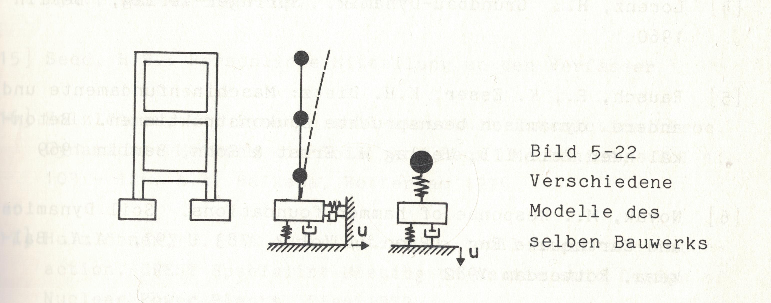
\includegraphics[width=\textwidth]{fig_pdf/haus1dof} 
%\caption*{aus \cite{haupt1986bodendynamik}}
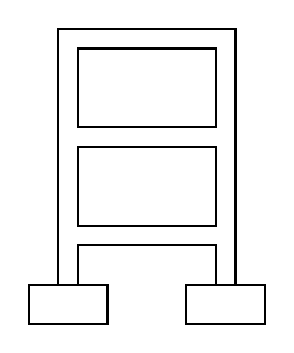
\begin{tikzpicture}
    \draw[black, thick] (-1.5,0) rectangle (-0.5, 0.5);
    \draw[black, thick] (1.5,0) rectangle (0.5, 0.5);
    \draw[black, thick] (-0.875, 1.25) rectangle (0.875,2.25);
    \draw[black, thick] (-0.875, 2.5) rectangle (0.875,3.5);
    \draw[black, thick] (-1.125, 0.5) -- (-1.125, 3.75) -- (1.125, 3.75) -- (1.125 ,0.5);
    \draw[black, thick] (-0.875, 0.5) -- (-0.875, 1) -- (0.875, 1) -- (0.875, 0.5);
\end{tikzpicture}
 % Rahmen

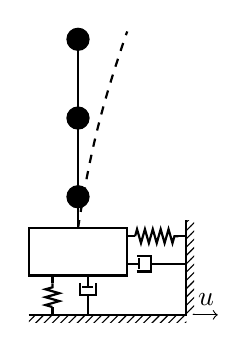
\begin{tikzpicture}
    \draw[black,thick] (0,0) -- (2, 0) -- (2, 1.2); 

    %Schraffur einfügen
    \fill[pattern = north east lines] (0, -0.1) rectangle (2, 0);
    \fill[pattern = north east lines] (2, 0) rectangle (2.1 , 1.2);

    \draw[black, thick] (0, 0.5) rectangle (1.25, 1.1);
    \draw[black, thick] (0.625, 1.1) -- (0.625, 3.5);

    %zigzag Linie, unten 
    \draw[black, thick] (0.3, 0.4) -- (0.3, 0.5);
    \draw[black, thick] (0.3, 0) -- (0.3, 0.1);
    \draw[black, thick, decorate, decoration = {zigzag, segment length = 1mm}] (0.3, 0.1) -- (0.3, 0.4);

    %neben zigzag, unten
    \draw[black, thick] (0.75, 0) -- (0.75, 0.25);
    \draw[black,thick] (0.75, 0.5) -- (0.75, 0.35);
    \draw[black,thick] (0.68, 0.35) -- (0.82, 0.35);
    \draw[black, thick] (0.65, 0.4) -- (0.65, 0.25) -- (0.85, 0.25) -- (0.85, 0.4);

    %zigzag Linie, rechts
    \draw[black, thick] (1.25 , 1.0) -- (1.35, 1.0);
    \draw[black, thick] (1.9, 1.0) -- (2.0, 1.0);
    \draw[black, thick, decorate, decoration = {zigzag, segment length = 1mm}] (1.35, 1.0) -- (1.9,1.0);
    
    %unterhalb zigzag rechts
    \draw[black, thick] (1.25 , 0.65) -- (1.4, 0.65);
    \draw[black, thick] (1.55, 0.65) -- (2.0 , 0.65);
    \draw[black, thick] (1.4, 0.72) -- (1.4, 0.58);
    \draw[black, thick] (1.37 , 0.55) -- (1.55 , 0.55) -- (1.55 , 0.75) -- (1.37, 0.75);
    
    %Kugeln
    \filldraw[black] (0.625, 3.5) circle (4pt);
    \filldraw[black] (0.625, 2.5) circle (4pt);
    \filldraw[black] (0.625, 1.5) circle (4pt);

    %bend line
    %\tikz[every to/ .style = {bend left}]
    \draw[black, thick, dashed, style = {bend left = 5}] (0.625, 1.1) to (1.25 , 3.6);

    \draw[->] (2.1, 0) -- (2.4, 0);
    \draw (2.25, 0.2) node {$u$};
\end{tikzpicture} % 3-Massen auf Fundament
\documentclass{article}
\usepackage{tikz}
\usetikzlibrary{patterns}
\usetikzlibrary{decorations.pathmorphing}

\begin{document}
    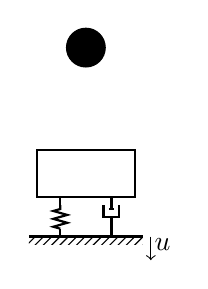
\begin{tikzpicture}
        \draw[black,thick] (-0.1,0) -- (1.35, 0);

        %Schraffur einfügen
        \fill[pattern = north east lines] (-0.1, -0.1) rectangle (1.35, 0);

        \draw[black, thick] (0, 0.5) rectangle (1.25, 1.1);

        %zigzag Linie, unten 
        \draw[black, thick] (0.3, 0.4) -- (0.3, 0.5);
        \draw[black, thick] (0.3, 0) -- (0.3, 0.1);
        \draw[black, thick, decorate, decoration = {zigzag, segment length = 1mm}] (0.3, 0.1) -- (0.3, 0.4);

        %neben zigzag, unten
        \draw[black, thick] (0.95, 0) -- (0.95, 0.25);
        \draw[black,thick] (0.95, 0.5) -- (0.95, 0.35);
        \draw[black,thick] (0.98, 0.35) -- (0.92, 0.35);
        \draw[black, thick] (0.85, 0.4) -- (0.85, 0.25) -- (1.05, 0.25) -- (1.05, 0.4);

        \draw[->] (1.45, 0) -- (1.45, -0.3);
        \draw (1.6, -0.1) node {$u$};

        %zigzag Linie, oben
        %\draw[black, thick] (0.625, 1.1) -- (0.625, 1.2);
        %\draw[black, thick] (0.625, 1.7) -- (0.625, 2);
        %\draw[black, thick, decorate, decoration = {zigzag, segment length = 1mm, amplitude = 2mm}] (0.625, 1.2) -- (0.625, 1.7);

        \filldraw[black] (0.625, 2.4) circle (7pt);

    \end{tikzpicture}
\end{document} % 1-Masse auf Fundament
\end{figure}
}

\end{frame}


\subsection{Freie Schwingungen}
\begin{frame}
\frametitle{Freie Schwingungen, {\normalsize ungedämpft}}
\begin{columns}
        \begin{column}[t]{.5\linewidth}
        \begin{figure}
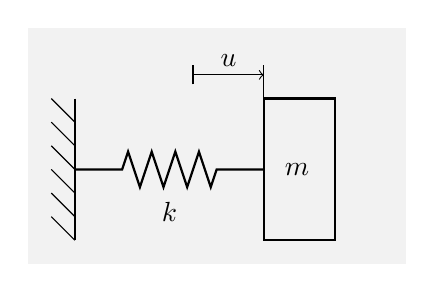
\begin{tikzpicture}[scale=0.6]
\fill[black!5!white] (-1,-2) rectangle (7, 3); 
\draw[->] (2.5, 2) --(4, 2);
\draw (2.5,1.8) -- (2.5, 2.2);
\draw[thin] (4,1.5)--(4,2.2);
\draw (0, 0) pic [scale=0.6] {DKbase};
\draw (0, 0) pic [scale=0.6, thick] {DKspring=4};  
\draw[thick] (4,-1.5) rectangle +(1.5, 3); 
\draw (2, -0.9) node {$k$};
\draw (4.7, 0) node {$m$};
\draw (3.25, 2.3) node {$u$};
\end{tikzpicture}


\uncover<2-5>{
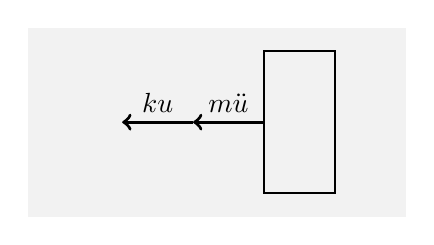
\begin{tikzpicture}[scale=0.6]
\fill[black!5!white] (-1,-2) rectangle (7, 2); 
\draw[thick] (4,-1.5) rectangle +(1.5, 3); 
\draw (3.25, 0.4) node {$m\ddot{u}$};
\draw (1.75, 0.4) node {$ku$};
\draw[<-, very thick] (2.5, 0) -- (4, 0);
\draw[<-, very thick] (1, 0) -- (2.5, 0);
\end{tikzpicture}

}
\caption*{Modell \uncover<2-5>{und Freischnitt}}
\end{figure}
        \end{column}
		\hfill
		\begin{column}[t]{.5\linewidth}
\uncover<3-5>{
		Bewegungsgleichung
\begin{equation*}
 -ku-m\ddot{u}=0
\end{equation*}
}
\uncover<4-5>{
Standardform
\begin{align*}
 \ddot{u}+\omega_0^2 u&=0\\
 \omega_0^2&=\frac{k}{m}
\end{align*}
}
\uncover<5>{
Lösung
\begin{equation*}
 u(t)=C_1\cos\omega_0 t + C_2\sin\omega_0 t
\end{equation*}
mit $C_1$, $C_2$ aus $u(t_0)=u_0$, $\dot{u}(t_0)=\dot{u}_0$
}
		\end{column}
\end{columns}
\end{frame}


\begin{frame}
\frametitle{Freie Schwingungen, {\normalsize gedämpft 1/5}}

\begin{columns}
        \begin{column}[t]{.5\linewidth}
        \begin{figure}
 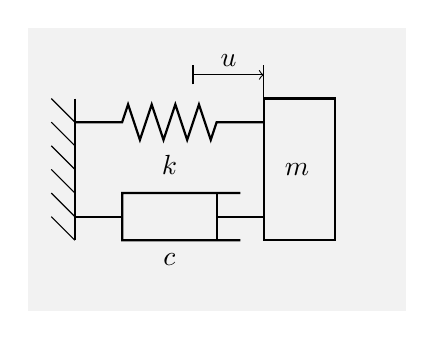
\begin{tikzpicture}[scale=0.6]
 \fill[black!5!white] (-1,-3) rectangle (7, 3); 
\draw (0, 0) pic [scale=0.6] {DKbase};
\draw (0, 1) pic [scale=0.6, thick] {DKspring=4};
\draw (0,-1) pic [scale=0.6, thick] {DKdashpot=4};  
\draw[->] (2.5, 2) --(4, 2);
\draw (2.5,1.8) -- (2.5, 2.2);
\draw[thin] (4,1.5)--(4,2.2);
\draw[thick] (4,-1.5) rectangle +(1.5, 3); 
\draw (2.0, 0.1) node {$k$};
\draw (2.0,-1.9) node {$c$};
\draw (4.7, 0) node {$m$};
\draw (3.25, 2.3) node {$u$};
\end{tikzpicture}


\uncover<2-4>{
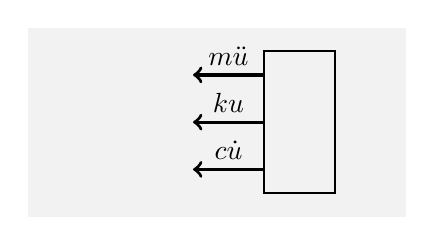
\begin{tikzpicture}[scale=0.6]
\fill[black!5!white] (-1,-2) rectangle (7, 2); 
\draw[thick] (4,-1.5) rectangle +(1.5, 3); 
\draw (3.25, 1.4) node {$m\ddot{u}$};
\draw (3.25, 0.4) node {$ku$};
\draw (3.25,-0.6) node {$c\dot{u}$};
\draw[<-, very thick] (2.5, 1) -- (4, 1);
\draw[<-, very thick] (2.5, 0) -- (4, 0);
\draw[<-, very thick] (2.5,-1) -- (4,-1);
\end{tikzpicture}

}
\caption*{Modell \uncover<2-4>{und Freischnitt}}
\end{figure}
        \end{column}
		\hfill
		\begin{column}[t]{.5\linewidth}
\uncover<3-4>{
		Bewegungsgleichung
\begin{equation*}
 -ku-c\dot{u}-m\ddot{u}=0
\end{equation*}
}
\uncover<4>{
Standardform
\begin{align*}
 \ddot{u}+2 \zeta\omega_0\dot{u}+\omega_0^2 u&=0\\
 2 \zeta\omega_0&=\frac{c}{m}\\
 \omega_0^2&=\frac{k}{m}
\end{align*}
}

		\end{column}
\end{columns}
\end{frame}


\begin{frame}
\frametitle{Freie Schwingungen, {\normalsize gedämpft 2/5}}
\begin{align*}
\ddot{u}+2 \zeta\omega_0\dot{u}+\omega_0^2 u&=0\\
u(t_0)&=u_0\\
\dot{u}(t_0)&=\dot{u}_0\\
\end{align*}
Gewöhnliche Differentialgleichung zweiter Ordnung mit konstanten Koeffizienten $\leadsto$ Exponentialansatz $u(t)=Ae^{\alpha t}$ $\leadsto$ charakteristische Gleichung
\begin{align*}
\alpha^2 + 2 \zeta\omega_0\alpha + \omega_0^2 &= 0 \\
\leadsto \alpha_{1}, \alpha_{2}&=- \zeta\omega_0\pm \omega_0\sqrt{ \zeta^2-1}
\end{align*}
\end{frame}


\begin{frame}
\frametitle{Freie Schwingungen, {\normalsize gedämpft 3/5}}
\begin{itemize}[<+->]

\item $\zeta^2>1$ überkritisch gedämpft, $\alpha_1, \alpha_2 \in \mathbb{R}$ und $\alpha_2 < \alpha_1 < 0$  
 \begin{equation*}
 u(t)=A_1 e^{\alpha_1 t}+ A_2 e^{\alpha_2 t}
 =A_1 e^{-\omega_0\left(\zeta-\sqrt{\zeta^2-1}\right)t}
 +A_2 e^{-\omega_0\left(\zeta+\sqrt{\zeta^2-1}\right)t}
 \end{equation*}
 
 \item $\zeta^2<1$ unterkritisch gedämpft, $\alpha_1, \alpha_2 \in \mathbb{C}$ und $\alpha_1=\bar{\alpha}_2$  
 \begin{equation*}
 u(t)= A_1 e^{\alpha_1 t}+ A_2 e^{\alpha_2 t}
 =e^{-\delta t}\bigl( C_1\cos\omega_1 t + C_2\sin\omega_1 t \bigr)
 \end{equation*}
 mit $\omega_1=\omega_0\sqrt{1- \zeta^2}$ und $\delta=\zeta\omega_0$, Herleitung folgt auf nächster Folie.
 
 \item $\zeta^2=1$ kritisch gedämpft,  $\alpha_1, \alpha_2 \in \mathbb{R}$ und $\alpha_1=\alpha_2<0$  
 \begin{equation*}
 u(t)= \bigl( A_1+A_2 t \bigr)e^{\alpha t}
 = \bigl( A_1+A_2 t \bigr)e^{-\zeta\omega_0 t}
 \end{equation*}
 Knobelspaß, siehe \textsl{mehrfache Nullstellen der charakteristischen Gleichung}!
\end{itemize}

\end{frame}

\begin{frame}
\frametitle{Freie Schwingungen, {\normalsize gedämpft 4/5}}
%Erinnerung Euler-Formel $e^{ix}=\cos x + i \sin x$ 
Herleitung der Lösung des unterkritisch gedämpften Falls
\begin{align*}
 u(t)  &=A_1 e^{-\omega_0\left( \zeta-\sqrt{ \zeta^2-1}\right)t}
  +A_2 e^{-\omega_0\left( \zeta+\sqrt{ \zeta^2-1}\right)t}\\
  &=A_1 e^{-\omega_0 \zeta t}e^{\omega_0 \sqrt{ \zeta^2-1}t}
  +A_2 e^{-\omega_0 \zeta t}e^{-\omega_0 \sqrt{ \zeta^2-1}t}\\
  &=A_1 e^{-\overbrace{\omega_0 \zeta}^{\delta} t}e^{i\overbrace{\omega_0 \sqrt{1-\zeta^2}}^{\omega_1}t}
  +A_2 e^{-\omega_0 \zeta t}e^{-i\omega_0 \sqrt{1-\zeta^2}t}\\
  &=A_1 e^{-\delta t}e^{i\omega_1t}+\mathrm{cc}(A_1) e^{-\delta t}e^{-i\omega_1t}\\
  &= e^{-\delta t}\Bigl( (A_{1R})+i A_{1I}) (\cos\omega_1 t + i \sin \omega_1 t  )\\
  & \qquad \quad +(A_{1R})-i A_{1I}) (\cos\omega_1 t - i \sin \omega_1 t)  \Bigr)\\
  &=e^{-\delta t}\bigl( \underbrace{2A_{1R}}_{C_1}\cos \omega_1 t 
  \underbrace{- 2A_{1R}}_{C_2}\sin \omega_1 t   \bigr)
 \end{align*}
\end{frame}


\begin{frame}
\frametitle{Freie Schwingungen, {\normalsize gedämpft 5/5}}

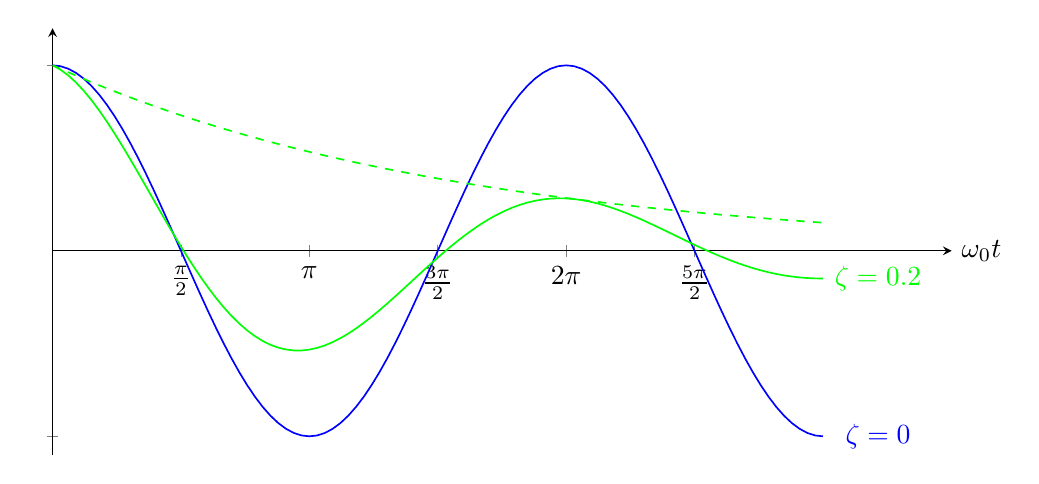
\begin{tikzpicture}
\begin{axis}[
    width=13cm, 
    height=7cm,
    axis x line=center, 
    axis y line=middle, 
    xlabel={$\omega_0 t$},
     x label style={at={(current axis.right of origin)}, right},
    samples=100,
    ymin=-1.1, ymax=1.2,
    xmin=0, xmax=11,
    domain=0:3*pi,
    xtick={ 1.5708, 3.14159, 4.7123889, 6.28318, 7.853981 },
    xticklabels={ 
    $\frac{\pi}{2}$, $\pi$, $\frac{3\pi}{2}$, $2\pi$, $\frac{5\pi}{2}$
    },
    ytick={-1,0,1},
    yticklabels={,,}
]
\addplot [mark=none, semithick, blue] {cos(deg(x))};
\addplot [mark=none, semithick, green, dashed] {exp(-0.2*x)};
\addplot [mark=none, semithick, green] {exp(-0.2*x)*cos(0.98*deg(x))};
\node[text=blue] at (axis cs:10.1,-1.0) {$\zeta=0$};
\node[text=green] at (axis cs:10.1,-0.15) {$\zeta=0.2$};
\end{axis}
\end{tikzpicture}


\end{frame}


%Einfach harmonisch

%Ungedämpfte
%Modell
%Bewergungsgleichung Lösung (fig)
% Resonanz Knobelspaß

%Gedämpfte
%FRF (fig A(f), phi(f))
%Knobelspaß 


\subsection{Erzwungene Schwingungen}
\begin{frame}
\frametitle{Erzwungene Schwingungen, {\normalsize ungedämpft 1/3}}
\begin{columns}
        \begin{column}[t]{.5\linewidth}
\begin{figure}
         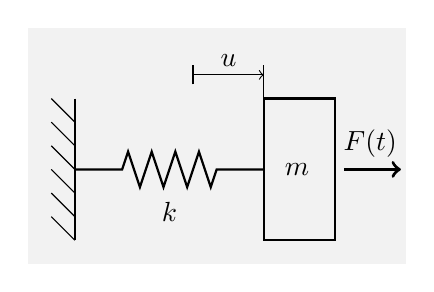
\begin{tikzpicture}[scale=0.6]
 \fill[black!5!white] (-1,-2) rectangle (7, 3); 
\draw[->] (2.5, 2) --(4, 2);
\draw (2.5,1.8) -- (2.5, 2.2);
\draw[thin] (4,1.5)--(4,2.2);
\draw (0, 0) pic [scale=0.6] {DKbase};
\draw (0, 0) pic [scale=0.6, thick] {DKspring=4};  
\draw[thick] (4,-1.5) rectangle +(1.5, 3); 
\draw (2, -0.9) node {$k$};
\draw (4.7, 0) node {$m$};
\draw (3.25, 2.3) node {$u$};
\draw[->, very thick] (5.7, 0) -- (6.9, 0);
\draw (6.25, 0.55) node {$F(t)$};
\end{tikzpicture}

        \uncover<2-4>{
        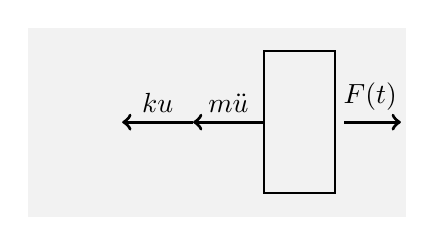
\begin{tikzpicture}[scale=0.6]
\fill[black!5!white] (-1,-2) rectangle (7, 2); 
\draw[thick] (4,-1.5) rectangle +(1.5, 3); 
\draw (3.25, 0.4) node {$m\ddot{u}$};
\draw (1.75, 0.4) node {$ku$};
\draw[<-, very thick] (2.5, 0) -- (4, 0);
\draw[<-, very thick] (1, 0) -- (2.5, 0);
\draw[->, very thick] (5.7, 0) -- (6.9, 0);
\draw (6.25, 0.55) node {$F(t)$};
\end{tikzpicture}

        }
        \caption*{Modell \uncover<2-4>{und Freischnitt}}
\end{figure}
        \end{column}
		\hfill
		\begin{column}[t]{.5\linewidth}
\uncover<3-4>{
		Bewegungsgleichung
\begin{equation*}
 F(t)-ku-m\ddot{u}=0
\end{equation*}
}
\uncover<4>{
Standardform
\begin{align*}
 \ddot{u}+\omega_0^2 u&=\omega_0^2 a(t)\\
 \omega_0^2&=\frac{k}{m}\\
 a(t)&= \frac{F(t)}{k}
\end{align*}
}
		\end{column}
\end{columns}
\end{frame}

\begin{frame}
\frametitle{Erzwungene Schwingungen, {\normalsize ungedämpft 2/3}}
\uncover<1-2>{
Die Gesamtlösung ist die Summe der Lösung der homogenen Gleichung (\textsl{Einschwingen}) und einer partikulären Lösung (\textsl{eingeschwungener Zustand})}
\begin{equation*}
 u(t)=u_h(t)+u_p(t).
\end{equation*}
Die Lösung der homogenen Gleichung entspricht der freien Schwingung. Um eine partikuläre Lösung für harmonische Anregung $F(t)=F_C\cos\omega t\uncover<1>{+F_S\sin\omega t}$ zu finden, wählen wir einen Ansatz vom Typ der rechten Seite
\begin{align*}
u_p(t)&=u_C\cos\omega t\uncover<1>{+u_S\sin\omega t},\\
\dot{u}_p(t)&=-u_C\omega\sin\omega t\uncover<1>{+u_S\omega\cos\omega t},\\
\ddot{u}_p(t)&=-u_C\omega^2\cos\omega t\uncover<1>{-u_S\omega^2\sin\omega t}.\\
\end{align*}
\uncover<2>{
Zunächst beschränken wir uns auf den Cosinus-Anteil (Sinus analog).}
\end{frame}


\begin{frame}
\frametitle{Erzwungene Schwingungen, {\normalsize ungedämpft 3/3}} 
\uncover<1-2>{
Einsetzen in die Bewegungsgleichung (Standardform) führt auf
\begin{equation*}
-u_C\omega^2\cos\omega t + u_C\omega_0^2\cos\omega t = a_C\omega_0^2\cos\omega t.
\end{equation*}
Koeffizientenvergleich liefert
\begin{equation*}
 u_C=\frac{\omega_0^2}{\omega_0^2-\omega^2}a_C
\quad \leadsto \quad 
 u_p(t)=\frac{1}{1-(\omega/\omega_0)^2}a_C \cos\omega t.
\end{equation*}
}
\uncover<2>{
Bei Resonanzanregung $\omega=\omega_0$ versagt dieser Ansatz, dann lautet die Lösung
\begin{equation*}
u_p(t)=\frac{\omega t}{2}\sin\omega t
\end{equation*}
Knobelspaß, siehe \textsl{Variation der Konstanten}!
}
\end{frame}


\begin{frame}
\frametitle{Erzwungene Schwingungen, {\normalsize gedämpft 1/5}}

\begin{columns}
        \begin{column}[t]{.5\linewidth}
        \begin{figure}
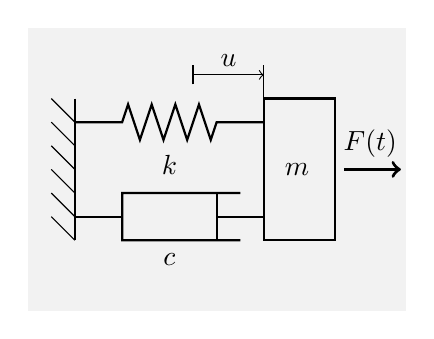
\begin{tikzpicture}[scale=0.6]
\fill[black!5!white] (-1,-3) rectangle (7, 3); 
\draw (0, 0) pic [scale=0.6] {DKbase};
\draw (0, 1) pic [scale=0.6, thick] {DKspring=4};
\draw (0,-1) pic [scale=0.6, thick] {DKdashpot=4};  
\draw[->] (2.5, 2) --(4, 2);
\draw (2.5,1.8) -- (2.5, 2.2);
\draw[thin] (4,1.5)--(4,2.2);
\draw[thick] (4,-1.5) rectangle +(1.5, 3); 
\draw (2.0, 0.1) node {$k$};
\draw (2.0,-1.9) node {$c$};
\draw (4.7, 0) node {$m$};
\draw (3.25, 2.3) node {$u$};
\draw[->, very thick] (5.7, 0) -- (6.9, 0);
\draw (6.25, 0.55) node {$F(t)$};
\end{tikzpicture}


\uncover<2-4>{
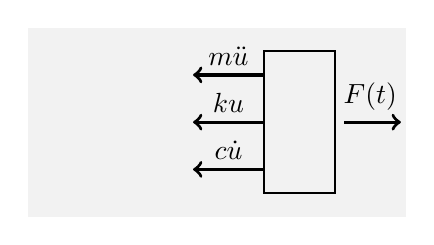
\begin{tikzpicture}[scale=0.6]
\fill[black!5!white] (-1,-2) rectangle (7, 2); 
\draw[thick] (4,-1.5) rectangle +(1.5, 3); 
\draw (3.25, 1.4) node {$m\ddot{u}$};
\draw (3.25, 0.4) node {$ku$};
\draw (3.25,-0.6) node {$c\dot{u}$};
\draw[<-, very thick] (2.5, 1) -- (4, 1);
\draw[<-, very thick] (2.5, 0) -- (4, 0);
\draw[<-, very thick] (2.5,-1) -- (4,-1);
\draw[->, very thick] (5.7, 0) -- (6.9, 0);
\draw (6.25, 0.55) node {$F(t)$};
\end{tikzpicture}

}
\caption*{Modell \uncover<2-4>{und Freischnitt}}
\end{figure}
        \end{column}
		\hfill
		\begin{column}[t]{.5\linewidth}
\uncover<3-4>{
		Bewegungsgleichung
\begin{equation*}
 F(t)-ku-c\dot{u}-m\ddot{u}=0
\end{equation*}
}
\uncover<4>{
Standardform
\begin{align*}
 \ddot{u}+2 \zeta\omega_0\dot{u}+\omega_0^2 u&=\omega_0^2 a(t)\\
 2 \zeta\omega_0&=\frac{c}{m}\\
 \omega_0^2&=\frac{k}{m}\\
  a(t)&= \frac{F(t)}{k}
\end{align*}
}
\end{column}
\end{columns}
\end{frame}


\begin{frame}
\frametitle{Erzwungene Schwingungen, {\normalsize gedämpft 2/5}}
Wie im ungedämpften Fall, und allgemein für jede inhomogene Differentialgleichung, gilt für die Gesamtlösung
\begin{equation*}
 u(t)=u_h(t)+u_p(t).
\end{equation*}
Für einfache harmonische Anregung $a(t)=a_C\cos\omega t + a_S \sin \omega t$
führt der Ansatz $u_p(t)=u_C\cos\omega t + u_S\sin\omega t$ auf
\begin{align*}
u_C&= V^2 \Bigl( (1-\eta^2)a_C-2\zeta\eta a_S \Bigl)\\
u_S&= V^2 \Bigl( (1-\eta^2)a_S+2\zeta\eta a_C \Bigl)
\end{align*}
Vergrößerungsfunktion $V=\frac{1}{\sqrt{(1-\eta^2)^2+(2\zeta\eta)^2}}$, \hfill Abstimmungsverhältnis $\eta= \frac{\omega}{\omega_0}$.
\smallskip
\begin{center}
 \textbf{Anmerkung:} der eingeschwungene Zustand für andere Anregungsarten (Dämpferfußpunkt-, Fundament-, Unwucht-) weist qualitative Unterschiede auf, die Herleitung verläuft aber analog.
\end{center}
\end{frame}

\begin{frame}
\frametitle{Erzwungene Schwingungen, {\normalsize gedämpft 3/5}}
Summen von Sinus- und Cosinusfunktionen lassen sich mittels
Additionstheoremen durch eine der beiden Funktionen darstellen
\begin{align*}
a(t)&= \hat{a}\cos(\omega t - \psi_a) = 
 \overbrace{\hat{a}\cos\psi_a}^{a_C} \cos(\omega t) +
 \overbrace{\hat{a}\sin\psi_a}^{a_S} \sin(\omega t).%\\
%u_p(t)&= \hat{u}\cos(\omega t - \psi_u) = 
% \hat{u}\cos\psi_u \cos(\omega t) +
% \hat{u}\sin\psi_u \sin(\omega t).
 \end{align*}
 Amplitude $\hat{a}$ und Phasenwinkel $\psi_a$ sind folglich festgelegt durch
 \begin{equation*}
  \hat{a}^2 = a_S^2+a_C^2 \qquad \text{und} \qquad
  \tan\psi_a = \frac{a_S}{a_C}. 
\end{equation*}
In dieser Darstellung lauten die Beziehungen zwischen Anregung und Antwort
\begin{equation*}
\frac{\hat{u}}{\hat{a}}=V \qquad \text{und} \qquad
\psi=\psi_u -\psi_a =  \frac{2\zeta\eta}{1-\eta^2}.
\end{equation*}

Anmerkung: Die Phasendifferenz wird üblicherweise auf $\psi\in(-\pi,\pi]$ begrenzt.
\end{frame}


\begin{frame}
\frametitle{Erzwungene Schwingungen, {\normalsize gedämpft 4/5}}

\only<1>{
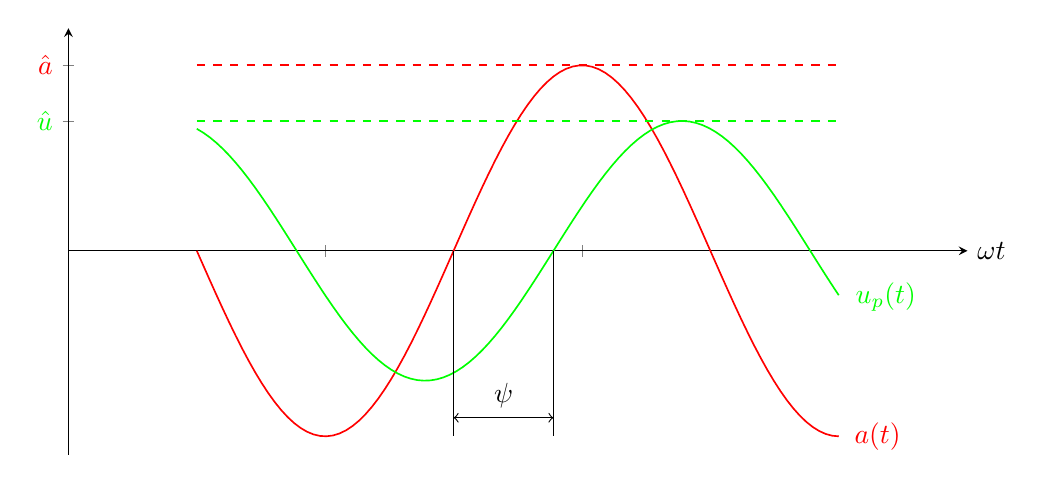
\begin{tikzpicture}
\begin{axis}[
    width=13cm, 
    height=7cm,
    axis x line=center, 
    axis y line=middle, 
    xlabel={$\omega t$},
     x label style={at={(current axis.right of origin)}, right},
    samples=100,
    ymin=-1.1, ymax=1.2,
    xmin=0, xmax=11,
    domain=0.5*pi:3*pi,
    xtick={   3.14159,  6.28318  },
    xticklabels={  ,  }, 
    ytick={0.7, 1},
    yticklabels={{\color{green}$\hat{u}$}, {\color{red} $\hat{a}$}}
]
\addplot [mark=none, semithick, red, dashed] {1};
\addplot [mark=none, semithick, red] {cos(deg(x))};
\addplot [mark=none, semithick, green, dashed] {0.7};
\addplot [mark=none, semithick, green] {0.7*cos(deg(x)-70)};
\node[text=red] at (axis cs: 9.9,-1.0) {$a(t)$};
\node[text=green] at (axis cs:10.0,-0.25) {$u_p(t)$};
\draw (axis cs: 4.712389, 0) -- (axis cs: 4.712389, -1);
\draw (axis cs: 5.934119, 0) -- (axis cs: 5.934119, -1);
\draw[<->] (axis cs: 4.712389, -0.9) -- node[above]{$\psi$} (axis cs: 5.934119, -0.9);
\end{axis}
\end{tikzpicture}

}

\only<2>{
\begin{figure}
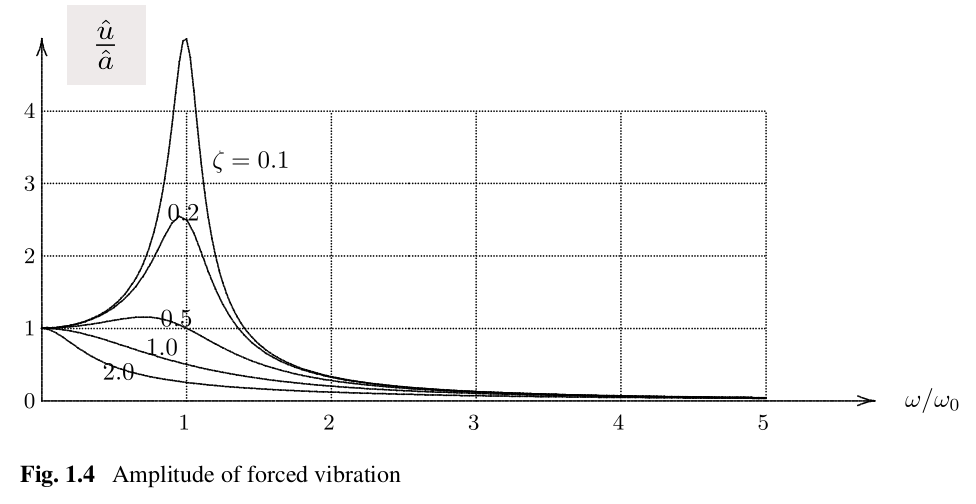
\includegraphics[width=0.9\textwidth]{fig_img/magnitude_response.png}
\caption*{aus \cite{Verruijt2010}}
\end{figure}
}

\only<3>{
\begin{figure}
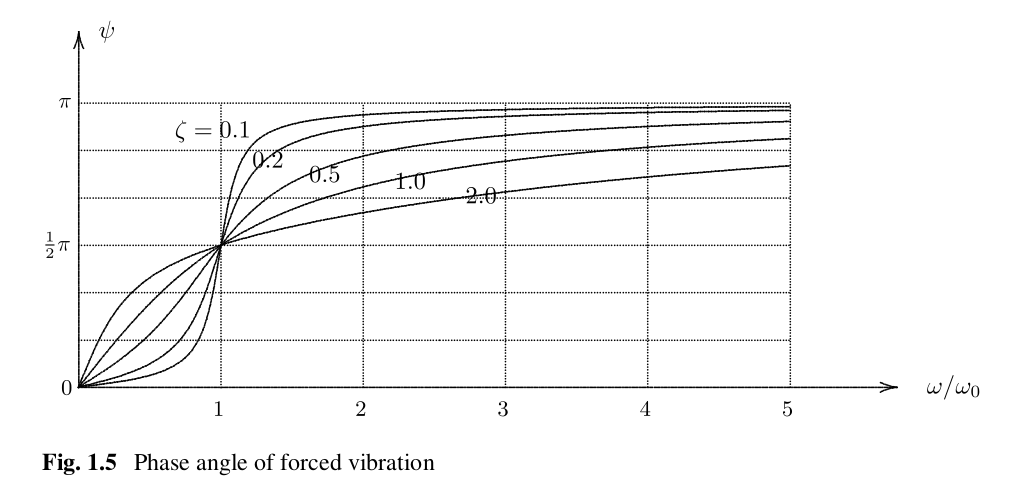
\includegraphics[width=\textwidth]{fig_img/phase_response.png}
\caption*{aus \cite{Verruijt2010}}
\end{figure}
}

\end{frame}

\begin{frame}
\frametitle{Erzwungene Schwingungen, {\normalsize gedämpft 5/5}}
Die Gesamtlösung lautet
\begin{equation*}
 u(t)=e^{-\delta t}\bigl( C_1\cos\omega_1 t + C_2\sin\omega_1 t \bigr)
 +u_C\cos\omega t + u_S\sin\omega t,
\end{equation*}
die unbestimmten Koeffizienten $C_1$ und $C_2$ folgen aus den Anfangsbedingungen
\begin{align*}
 u(t_0)&=u_0,\\
 \dot{u}(t_0)&=\dot{u}_0.
\end{align*}
\end{frame}


%%%%%%%%%%%%%%%%%%%%%%%%%%%%%%%%%%%%%%%%%%%%%%%%

\section*{Literaturverzeichnis}

\begin{frame}[allowframebreaks]{}
	\printbibliography
\end{frame}

\end{document}
